\chapter{Propuesta escalable de control In-band para entornos inalámbricos y de baja capacidad}
\label{ch:propuestaInband}

En este capítulo se presenta la primera aportación de la Tesis: una propuesta de control \textit{in-band} escalable para redes \gls{sdn} en entornos inalámbricos y de baja capacidad, concebida en el marco de los futuros ecosistemas \gls{6g}. El origen de esta línea de trabajo se remonta a mi Trabajo Fin de Máster~\cite{carrascal2023diseno}, donde se sentaron las primeras bases conceptuales. Posteriormente, se consolidó mediante el desarrollo y publicación de una revisión sistemática sobre los mecanismos de control \gls{sdn} \textit{in-band}~\cite{carrascal2023comprehensive}, y materializó como primera contribución de la Tesis en forma de ponencia en la conferencia CommNet 2023~\cite{carrascal2023scalable}. Aunque la evaluación experimental de esta propuesta se planteó principalmente como una prueba de concepto y, por tanto, no resulta exhaustiva, constituye un punto de partida sólido que guía y fundamenta las siguientes contribuciones de la Tesis.

\section{Introducción}

Los recientes avances en comunicaciones móviles, junto con la mejora de las capacidades de hardware, han impulsado el crecimiento del \gls{iot} al interconectar miles de millones de objetos mediante comunicaciones \gls{m2m} en entornos tanto domésticos como industriales~\cite{Balaji2019}. Puede afirmarse sin lugar a dudas que el \gls{iot} forma parte integral del Internet presente y futuro: ha transformado la forma en que interactuamos con el entorno, permitiendo la interconexión autónoma de dispositivos a través de la red y ofreciendo entornos inteligentes y adaptativos que responden a las necesidades de la sociedad. No obstante, el crecimiento exponencial de dispositivos \gls{iot} conectados a redes móviles introduce nuevas exigencias en términos de capacidad, rendimiento, latencia y eficiencia de red que deben abordarse (Ver Figura~\ref{fig:in_band_1}). La tecnología \gls{5g} se propuso y desplegó comercialmente para cubrir muchos de los requisitos de las redes \gls{iot} y sus aplicaciones. Sin embargo, con la rápida proliferación de nuevos sensores y la consiguiente expansión de las redes \gls{iot}, los requisitos técnicos necesarios para sostener los entornos tradicionales \gls{m2m} (plenamente autónomos, dinámicos e inteligentes) se han incrementado. Por tanto, se requiere una tecnología más avanzada para satisfacer las demandas futuras de las redes \gls{iot}, y la arquitectura \gls{6g} se postula como una solución capaz de afrontar estos nuevos retos~\cite{Nguyen2022}.

\begin{figure}[ht!]
   \centering
    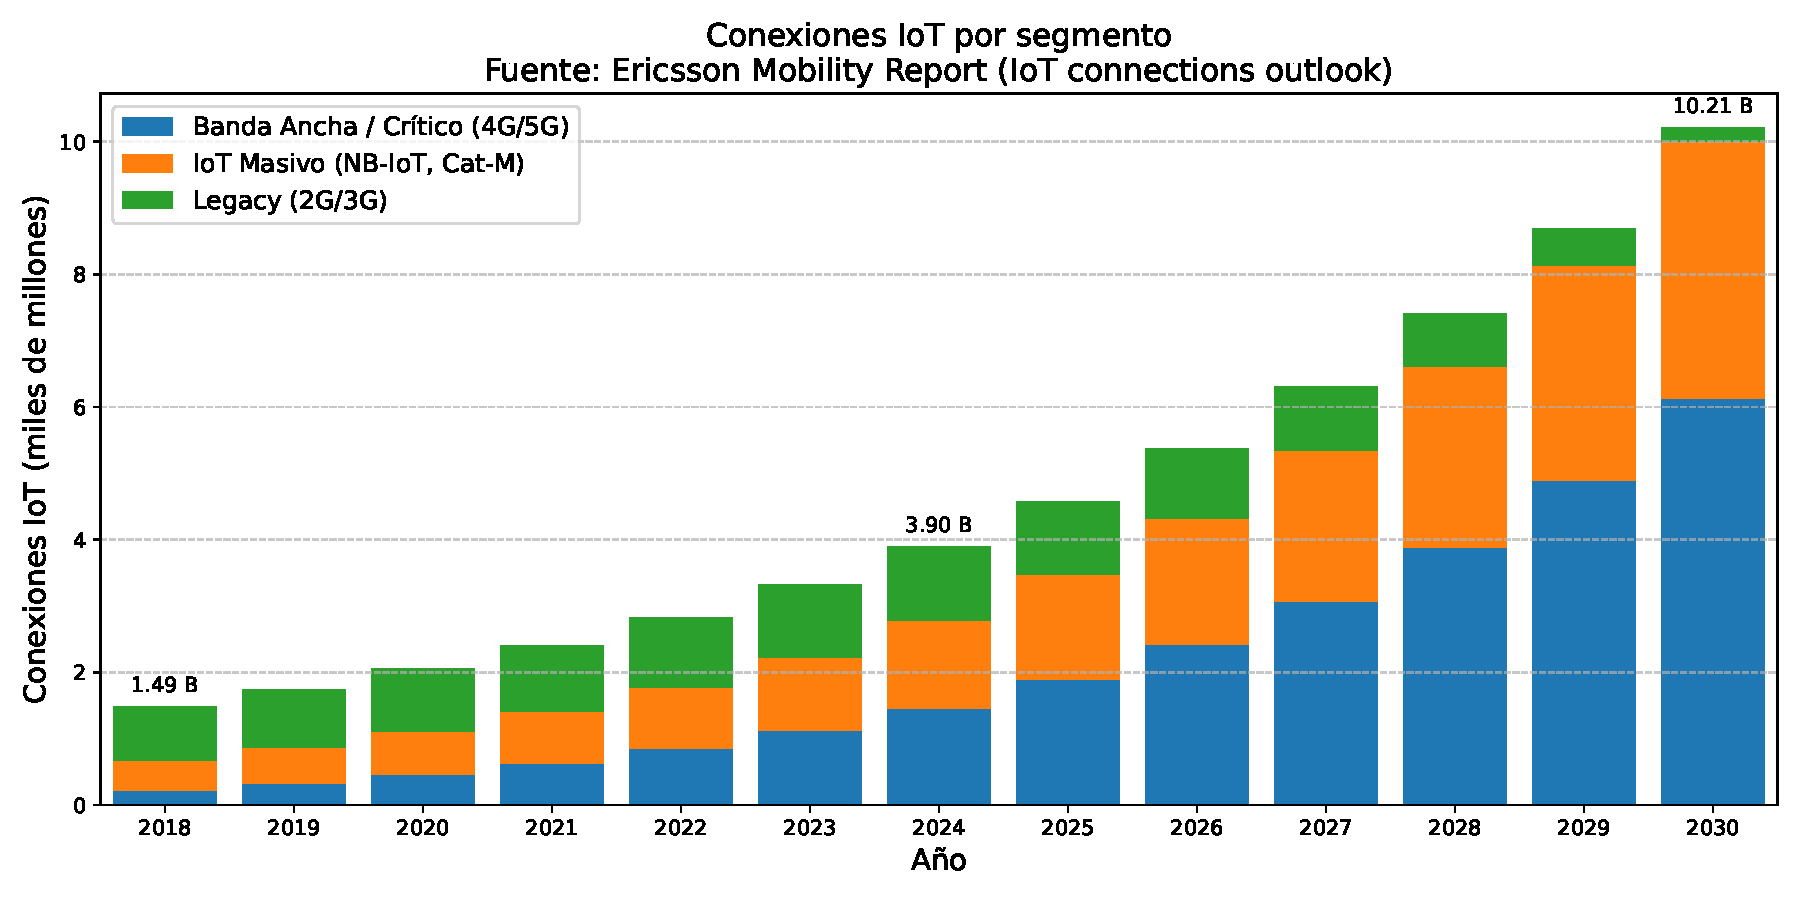
\includegraphics[width=\textwidth]{fig/04_in-band/in_band_1.pdf}
    \caption{Estudio del crecimiento de las conexiones de dispositivos IoT desglosadas por segmento~\cite{ericsson2025_iot}.}
    \label{fig:in_band_1}
\end{figure}


Un aspecto esencial de la nueva generación de redes móviles es la arquitectura de interconexión física que se propondrá. En \gls{5g}, la columna vertebral \gls{sdn} existente (en las redes móviles anteriores) se reutilizó incorporando modificaciones software para acomodar las nuevas especificaciones arquitectónicas mediante flexibilidad y programabilidad~\cite{Li2018}. En esta línea, cabe preguntarse si la futura red \gls{6g} aprovechará los beneficios de \gls{sdn} para el procesamiento de datos en su backbone. Los informes preliminares sobre el diseño de \gls{6g}~\cite{uusitalo20216g,6garch1,6garch2} indican que \gls{sdn}, junto con tecnologías como \gls{p4} y técnicas de \gls{ai}/\gls{ml}, se emplearán para definir el plano de procesamiento de datos y mejorar el rendimiento y la orquestación de la infraestructura existente. Además, las redes \gls{6g} enfatizarán la necesidad del paradigma \gls{mec}, extendiendo el borde de la red hacia los usuarios y construyendo el llamado continuo \textit{edge-to-cloud} (o simplemente \textit{cloud continuum})~\cite{Milojicic20}. Aunque \gls{sdn} sigue siendo un pilar del \textit{edge computing}, existen aún desafíos en la integración de \gls{iot} y \gls{sdn} en el borde de la red~\cite{Bittencourt18}, tales como la adaptación de estándares y recomendaciones \gls{sdn} a entornos inalámbricos, y la compatibilidad con dispositivos heterogéneos y con recursos restringidos, característicos de las redes \gls{iot} (Según se ha analizado en el Capítulo~\ref{ch:problema}).\\
\\
En el caso específico del plano de control \gls{sdn}, se consideran dos paradigmas de control: \textit{out-of-band} e \textit{in-band} (Según se estudió en la Sección~\ref{subsec:arquitectura_fisica_sdn}). Mientras que en el enfoque \textit{out-of-band} cada nodo \gls{sdn} dispone de un enlace dedicado al controlador (es decir, la información de control circula por una red dedicada), en el modelo \textit{in-band} sólo ciertos nodos gestionados cuentan con enlace directo al controlador y el resto de dispositivos reutilizan dichos enlaces para reenviar la información de control hacia el \gls{sdn} controller (la información de control, al no disponer de una red dedicada, viaja conjuntamente con el tráfico de datos hasta alcanzar el controlador). Aunque no existe un paradigma de control intrínsecamente superior, cada enfoque tiene ventajas e inconvenientes y la elección depende del caso de uso concreto, los dispositivos \gls{iot} con recursos restringidos en el extremo de la red se benefician en general del control \textit{in-band}: aunque potencialmente menos seguro~\cite{feghali2015sdn}, sus requisitos computacionales y energéticos suelen ser inferiores. No obstante, según se revisó (Sección~\ref{subsec:conclu_inband}), no existe un estándar específico que defina el control \textit{in-band}; y, si bien existen propuestas en la literatura, pocas contemplan entornos inalámbricos y ninguna está diseñada explícitamente para dispositivos con recursos limitados.\\
\\
En este capítulo se presenta, \texttt{win-BOFUSS}, una solución evolucionada del switch \gls{bofuss} que soporta control \textit{in-band} para escenarios inalámbricos, diseñada de forma escalable y orientada a dispositivos \gls{iot}.

\section{Descripción del protocolo}
\label{sec:inband_proto_desc}
El Estado del Arte ha puesto de manifiesto que el etiquetado jerárquico y las técnicas basadas en árboles enraizados constituyen un marco fértil y consolidado para abordar el arranque y la provisión de canales de control en entornos densos y heterogéneos (Ver Sección~\ref{subsubsec:conclu_etiquetado}). Las propuestas revisadas comparten la idea de explotar información codificada localmente en etiquetas para reducir estado y facilitar encaminamiento hacia la raíz o raíces. Es por ello, que nuestro protocolo \textit{in-band} busca y establece múltiples rutas entre un nodo raíz y el resto de los nodos de la topología, creando múltiples árboles conectados. La novedad de este protocolo es que permite al controlador \gls{sdn} comunicarse mediante canales \textit{in-band} en entornos inalámbricos, lo cual no es común dado que \gls{sdn} fue diseñado originalmente para escenarios cableados. 
Existen propuestas enfocadas de etiquetado jerárquico en redes \gls{llns} (IoTorii, de Rojas \textit{et al.}~\cite{rojas2021outperforming}), que al igual que esta solución, están concebidas para requerir pocos recursos computacionales y de memoria en dispositivos restringidos, sin embargo, esta propuesta habilita a los nodos \gls{iot} interactuar de forma nativa en entornos \gls{sdn}. Por lo tanto, resulta particularmente adecuado para redes \gls{iot}-\gls{sdn}. Asimismo, gracias a la funcionalidad \textit{multipath} que ofrece el protocolo, también es posible almacenar diferentes rutas de respaldo que pueden utilizarse en caso de fallos o en escenarios de movilidad dentro del área de cobertura, manteniendo siempre activa la sesión con el controlador.\\
\\
La definición de este protocolo se apoya en el trabajo de Constantin \textit{et al.}~\cite{constantin2020desarrollo}, en el que se establecen múltiples rutas entre un nodo raíz y el resto de nodos de la topología en un escenario cableado. Estas múltiples rutas se construyen combinando dos técnicas (según se explicaba en la Sección~\ref{subsubsec:teminologia_grafos}): el etiquetado jerárquico de los dispositivos y una inundación controlada de dichas etiquetas. En primer lugar, se selecciona un nodo raíz de la red (generalmente un nodo con acceso al controlador \gls{sdn}), y dicho nodo genera un mensaje inicial con una etiqueta específica que envía a sus nodos directamente conectados. El dispositivo receptor inunda este mensaje a sus vecinos a través de todas las interfaces excepto aquella por la que recibió el mensaje. Además, añade un nuevo elemento a la etiqueta recibida por cada interfaz de salida con el fin de rastrear la ruta recorrida a lo largo de la topología. Cada vecino que recibe el mensaje repetirá este proceso. El proceso de inundación puede detenerse en cualquier nodo considerando parámetros específicos de la etiqueta recibida, tales como la longitud de la etiqueta, el prefijo común de la etiqueta, entre otros. Eventualmente, cada nodo recibirá un conjunto de etiquetas jerárquicas que identifican múltiples rutas para alcanzar el nodo raíz (quien envió la primera etiqueta) desde el nodo actual. Si el nodo raíz es un nodo conectado al controlador \gls{sdn}, entonces cada nodo podrá establecer comunicación con el controlador a través de cualquiera de esas rutas etiquetadas. Estas etiquetas reciben el nombre de \gls{hlmac}, siguiendo la idea del estándar IEEE 802c-2017~\cite{ieee802c2017}, que define el uso de direcciones \gls{mac} locales. \\
\\
Nuestro protocolo adapta la idea original a entornos inalámbricos. El reto principal en estos escenarios es que, a diferencia de las redes cableadas, los dispositivos inalámbricos suelen disponer de una única interfaz radio que les permite comunicarse con todos los vecinos dentro de su área de cobertura; por tanto, el mecanismo de etiquetado jerárquico propuesto en~\cite{constantin2020desarrollo} no puede aplicarse directamente. Para solventar esta limitación incorporamos conceptos tomados de IoTorii de Rojas \textit{et al.}~\cite{rojas2021outperforming} (una línea de trabajo en la que participé antes del Doctorado) y adaptamos el etiquetado a la naturaleza broadcast del medio inalámbrico. Concretamente, el proceso se basa en identificar previamente los vecinos que se encuentran realmente en rango de cobertura y, sobre esa información local, asignar las etiquetas jerárquicas correspondientes en función de la relación de vecindad (y no del puerto de salida). De este modo cada nodo construye su vista local del entorno y puede generar/propagar etiquetas coherentes para el encaminamiento en topologías inalámbricas. \\
\\
Por tanto, el protocolo se basa en dos procesos fundamentales que operan de forma complementaria:

\begin{itemize}

\item \textbf{Reconocimiento de vecindad} (Detallado en la sub-Sección~\ref{subsubsec:procesoVecinos}): Mecanismo local y periódico mediante el cual cada nodo detecta y mantiene la lista actualizada de vecinos en rango (tabla de vecinos). Esta información sirve para identificar enlaces activos, eliminar vecinos “muertos” y proporcionar la base para la asignación de identificadores locales que sustituyen al concepto de puerto físico en entornos cableados.

\item \textbf{Etiquetado jerárquico} (Detallado en la sub-Sección~\ref{subsubsec:procesoEtiquetado}): Proceso de generación y difusión controlada de etiquetas (\gls{hlmac}) que permite construir uno o varios árboles enraizados en los nodos con acceso al controlador \gls{sdn}. El etiquetado utiliza la información de vecindad para propagar rutas jerarquizadas, reducir el estado por nodo y habilitar encaminamiento multipath y protección ante fallos o movilidad.

\end{itemize}

\subsection{Proceso de reconocimiento de vecindad}
\label{subsubsec:procesoVecinos}

El proceso de reconocimiento de vecindad es un proceso ligero y periódico cuya función es mantener, en cada nodo, una tabla de vecinos con entradas de tipo tuplas, donde se asocia cada dirección \gls{mac} vecina con un identificador local (ID). Esta tabla se actualiza  localmente en cada nodo mediante mensajes \textit{Hello}, que cada nodo difunde periódicamente en su área de cobertura. Por tanto, los objetivos del proceso de reconocimiento de vecindad son los siguientes:

\begin{itemize}
    \item Detectar vecinos nuevos. Al recibir un mensaje \textit{Hello}, el nodo inspecciona la dirección \gls{mac} remitente; si no está presente en la tabla de vecinos, se crea una nueva entrada almacenando la asociación \((MAC \rightarrow ID)\). La ID puede generarse como un contador incremental (sufijo) o mediante otro esquema determinista según la implementación.
    
    \item Detectar vecinos ``muertos''. Cada entrada en la tabla incorpora un temporizador (\textit{timeout}) que se refresca al recibir \textit{Hello} periódicos del vecino correspondiente. Si el temporizador expira, la entrada se elimina y se invalidan las rutas que dependieran de dicho vecino, asumiendo una ausencia por fallo o movilidad.
    
    \item Parametrización y control de señalización. El periodo de emisión de mensajes tipo \textit{Hello} y los umbrales de \textit{timeout} son parámetros configurables que permiten adaptar el coste de señalización a la densidad y movilidad del despliegue (p. ej., intervalos más largos en redes muy densas o donde la energía es limitada).
    
    \item Escalabilidad local. El mecanismo está diseñado para que la carga por nodo dependa principalmente de su grado de conectividad (número de vecinos). Esto facilita dimensionar recursos (memoria, CPU) y ajustar parámetros en dispositivos con capacidades limitadas.
\end{itemize}



Desde el punto de vista de coste, el mecanismo es muy simple: por cada ronda de descubrimiento, cada nodo emite un \textit{Hello} y recibe tantos \textit{Hello} como grado local de conectividad tenga. Esta caracterización ayuda a dimensionar el periodo de \textit{Hello} y el tiempo de expiración (\textit{timeout}) en función de la densidad y movilidad del despliegue.\\
\\
Para ilustrar este proceso, se presenta la Figura~\ref{fig:in_band_2}. Según se puede apreciar en el inferior de la Figura, se ha ejemplificado una topología inalámbrica de ejemplo, donde los enlaces representados indican que ambos nodos se encuentran en radio de cobertura. Tomando la Figura~\ref{fig:in_band_2} como ejemplo, podemos observar cómo se rellenarían las tablas de vecinos una vez el proceso hubiera convergido. En el caso del nodo \textit{A}, sólo detecta al nodo \textit{B} y almacenará la entrada \((\text{MAC}_B,\; \text{ID}=1)\). El nodo \textit{B} detecta a \(\{A,C,D\}\) y asigna tres IDs locales \(\{1,2,3\}\) respectivamente; \textit{C} registra a \(\{B,F\}\) con dos IDs, y así de forma análoga. Nodos con alta conectividad (p. ej. \textit{B} o \textit{D}) soportan mayor carga de recepción y mantienen más entradas, lo que debe tenerse en cuenta al dimensionar recursos en dispositivos con capacidades limitadas.\\
\\
Es por ello que, el proceso de reconocimiento de vecindad, apoyado en los mensajes \textit{Hello} y la tabla de vecinos proporcionan una base local, eficiente y fácilmente parametrizable para habilitar el etiquetado jerárquico y la construcción de árboles en entornos inalámbricos y móviles, controlando explícitamente el intercambio de señalización en función de la densidad y la movilidad de la red.

\begin{figure}[ht!]
    \centering
    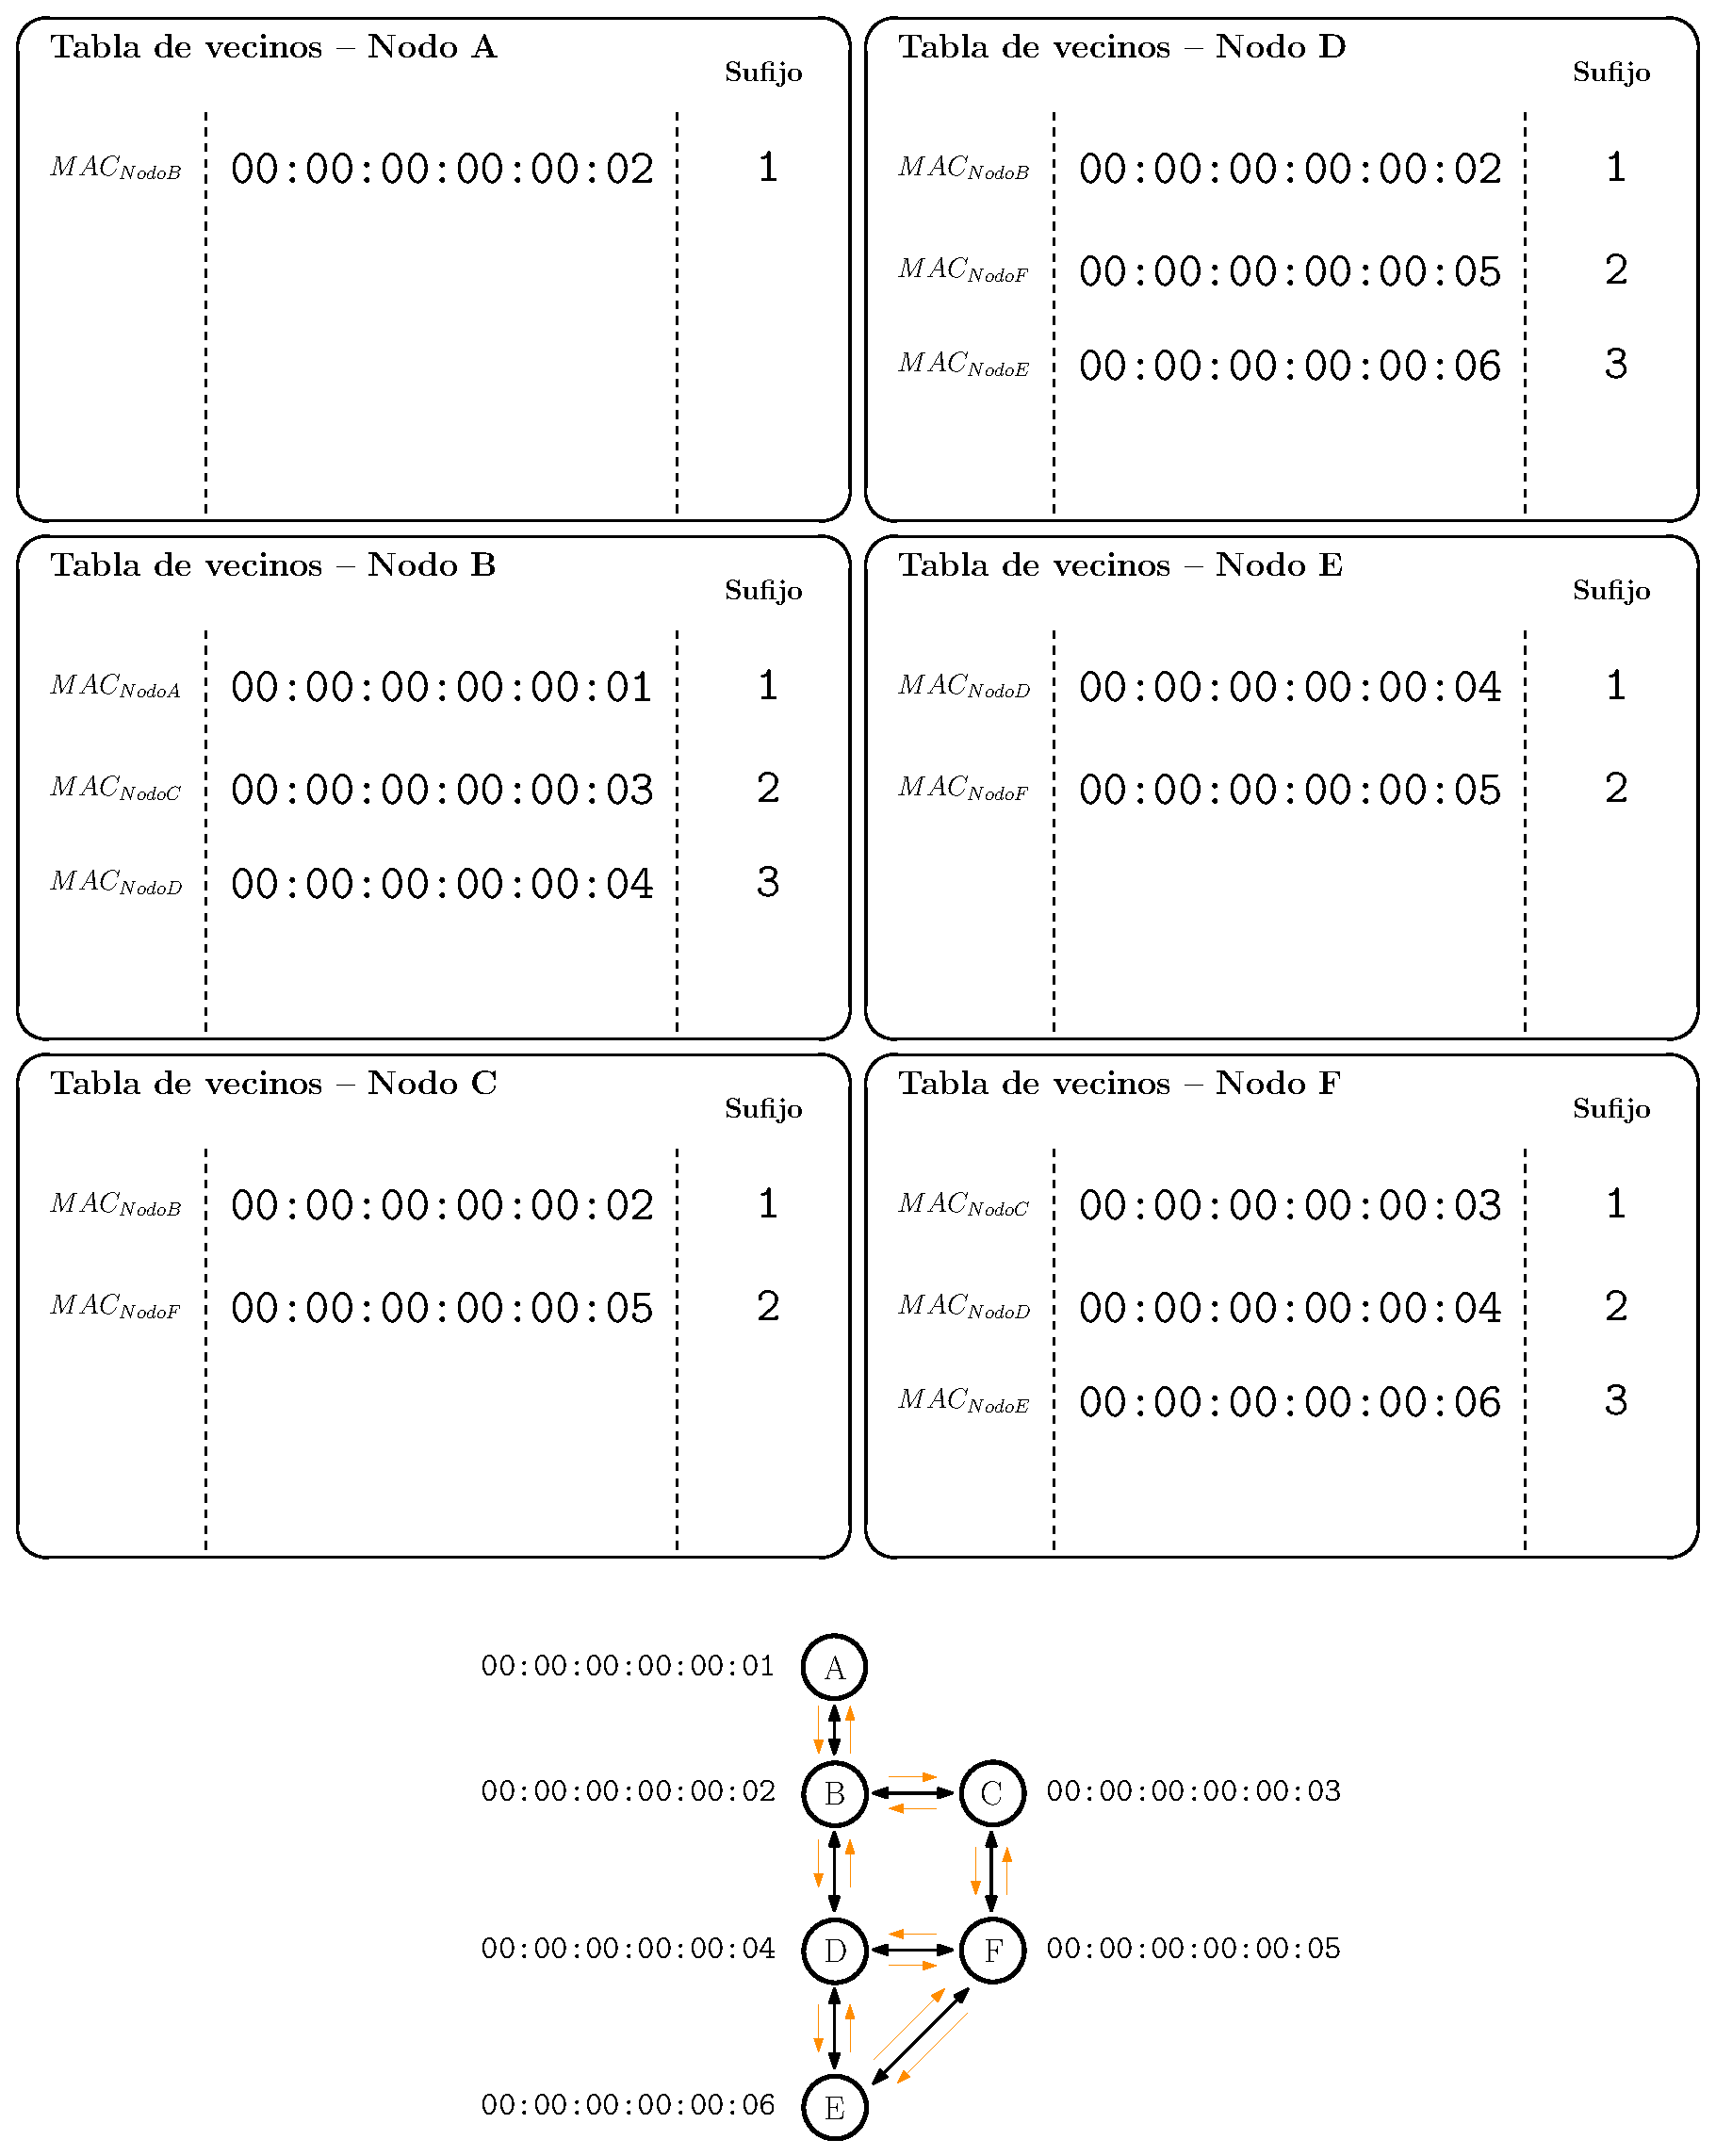
\includegraphics[width=\textwidth]{fig/04_in-band/in_band_2.eps}
    \caption{Proceso de reconocimiento de vecindad empleando las tablas locales de vecinos.}
    \label{fig:in_band_2}
\end{figure}

\subsection{Proceso de etiquetado jerárquico}
\label{subsubsec:procesoEtiquetado}

Una vez se ha explicado el proceso de reconocimiento de vecindad en la topología inalámbrica, se va a detallar el proceso de etiquetado jerárquico del protocolo. Para ilustrar y aclarar el proceso de construcción de la topología lógica a partir de la topología física, la Figura~\ref{fig:in_band_3} muestra el proceso de inundación de las \gls{hlmac} en una topología de ejemplo de seis nodos, donde el nodo \textit{A} actúa como nodo raíz (el que tendrá acceso con el controlador \gls{sdn}). El procedimiento arranca después de haberse intercambiado al menos una ronda de paquetes \textit{Hello}, es decir, cuando todos los nodos conocen a sus vecinos y han poblado sus tablas locales de vecinos con la asociación dirección \((MAC \rightarrow ID)\). Las áreas de cobertura y las relaciones de vecindad se representan con una flecha doble negra (por ejemplo, \textit{B} tiene por vecinos a \textit{A}, \textit{C} y \textit{D}). La figura se divide en cuatro subfiguras que representan pasos sucesivos del procedimiento.\\
\\
La Fig.~\ref{fig:in_band_3}(a) ilustra el primer paso del proceso: el nodo \textit{A} envía la primer \gls{hlmac}, que es recibida por el nodo \textit{B}. La \gls{hlmac} inicial enviada por \textit{A} está compuesta por el ID de \textit{A} y por el ID local que \textit{A} asignó a \textit{B}, representado como \textit{1.1}. Concretamente, \textit{A} sabe por el intercambio previo de los mensajes \textit{Hello} que sólo tiene un vecino (\textit{B}) y le asigna el ID \textit{1}. Cuando \textit{B} recibe \textit{1.1}, consulta su tabla local de vecinos y comprueba que tiene tres vecinos [\textit{A,C,D}] con ID locales [\textit{1,2,3}]. En ese contexto, \textit{A} se considera el nodo padre (que fue quien envió el \gls{hlmac} inicial) y \textit{C}, \textit{D} son nodos hijos. A continuación, \textit{B} genera dos nuevas \gls{hlmac}, \textit{1.1.2} y \textit{1.1.3}, y las envía a \textit{C} y \textit{D}, respectivamente; pero no se envía \gls{hlmac} al nodo padre. Es importante subrayar que no se inundan todos los nodos con \gls{hlmac} para evitar bucles: sólo se retransmiten aquellas \gls{hlmac} que no sean extendidas de una \gls{hlmac} previamente almacenada como hija. Por ejemplo, si \textit{B} ya ha guardado \textit{1.1} y en una iteración posterior recibe una \gls{hlmac} del tipo \textit{1.1.x...}, la descartará inmediatamente porque proviene de uno de sus hijos y por tanto representaría un bucle.\\
\\
La Fig.~\ref{fig:in_band_3}(b) muestra el segundo paso: las \glspl{hlmac} enviadas por \textit{B} (\textit{1.1.2} y \textit{1.1.3}) son recibidos por los nodos \textit{C} y \textit{D}. El nodo \textit{C} verifica que tiene dos vecinos [\textit{B,F}] con IDs [\textit{1,2}] y, por tanto, sólo genera y reenvía la \gls{hlmac} \textit{1.1.2.2} hacia su hijo \textit{F}. En el caso del nodo \textit{D}, con vecinos [\textit{B,F,E}] e IDs [\textit{1,2,3}] (donde \textit{F} y \textit{E} son hijos), produce \textit{1.1.3.2} y \textit{1.1.3.3} y las reenvía a \textit{E} y \textit{F}. El proceso se repite en \textit{E} y \textit{F}, tal y como se muestra en la Fig.~\ref{fig:in_band_3}(c), donde las nuevas \glspl{hlmac} aprendidas por cada nodo se resaltan en negrita. La subfigura inferior derecha (Fig.~\ref{fig:in_band_3}(d)) recoge el conjunto final de \glspl{hlmac} almacenadas en todos los nodos de la topología.\\
\\
Al finalizar el procedimiento, cada nodo habrá almacenado múltiples \glspl{hlmac}, es decir, varias rutas posibles hacia la raíz. Por ejemplo, \textit{B} sólo tendrá un \gls{hlmac} (una única ruta hacia la raíz), mientras que \textit{C}, \textit{D} y \textit{F} dispondrán de tres \glspl{hlmac} (tres rutas hacia el nodo raíz) y \textit{E} de cuatro \glspl{hlmac}, teniendo más opciones para alcanzar al nodo que da acceso al controlador \gls{sdn}. Además, el número total de \glspl{hlmac} por nodo puede limitarse a un valor prefijado, de modo que cada nodo mantenga como máximo un número de rutas, lo que representa una tensión entre cantidad de información de estado por nodo contra la capacidad de resiliencia con rutas de respaldo a nivel de nodo. 

\begin{figure}[ht!]
     \centering
     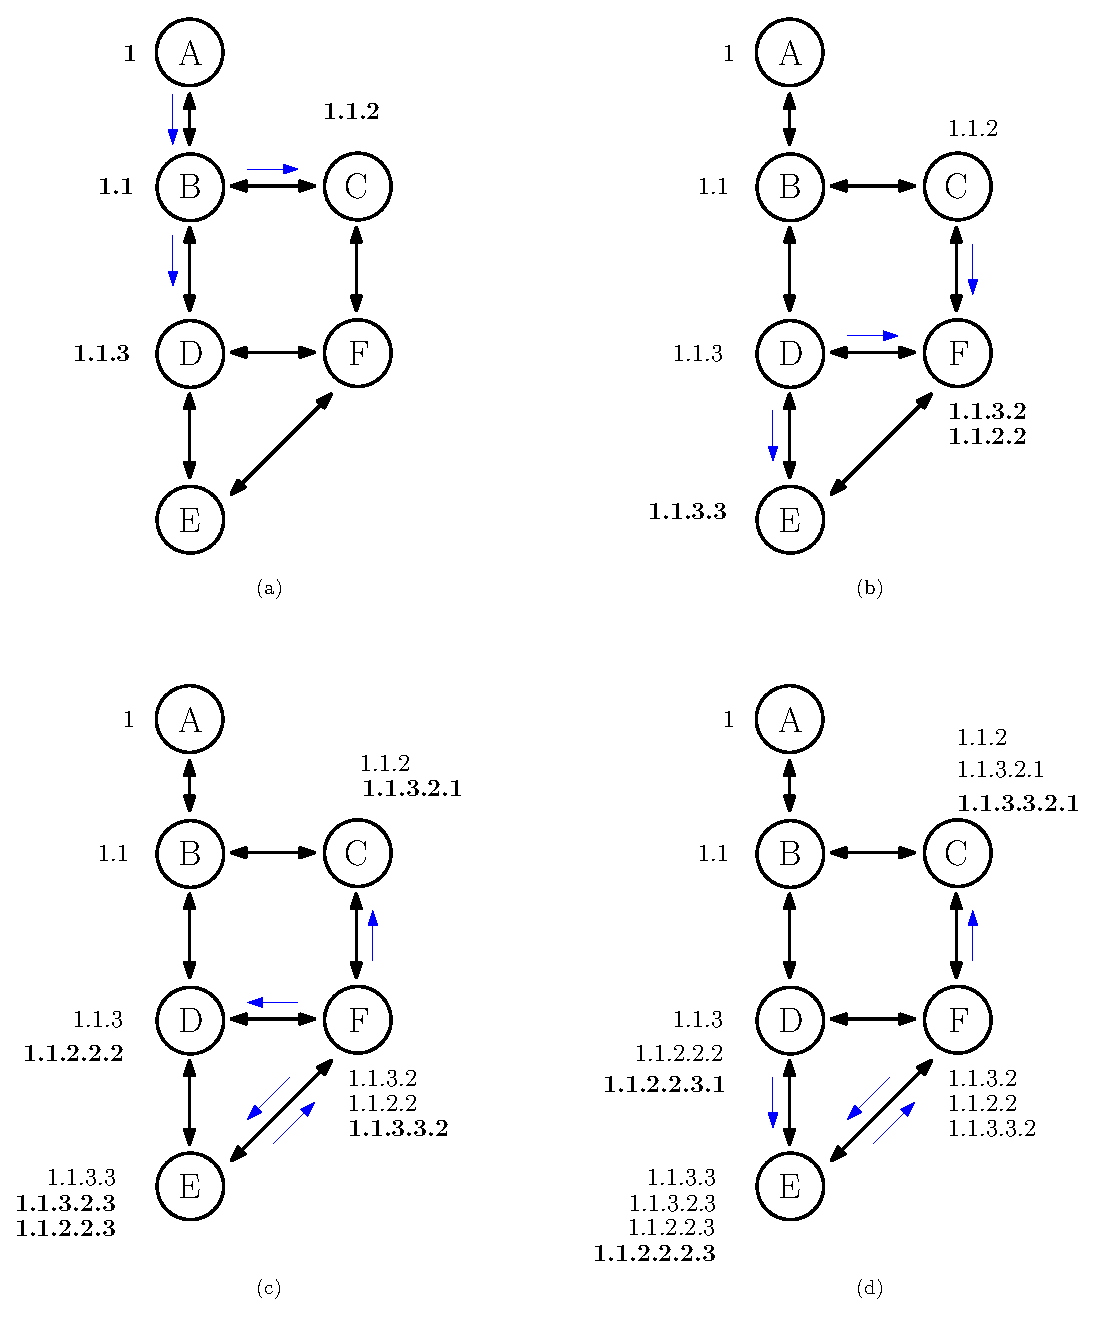
\includegraphics[width=\textwidth]{fig/04_in-band/in_band_3.eps}
     \caption{Proceso de difusión de etiquetas Hierarchical Local MAC (HLMAC) en la topología de ejemplo.}
     \label{fig:in_band_3}
\end{figure}

La elección de que ruta utilizar depende de criterios del caso de uso final, y de las características propias de la topología, pudiendo optar por el menor número de saltos, menor latencia, máxima redundancia, entre otros. En este caso, al ser una prueba de concepto, no se ha explorado en profundidad el impacto de los criterios, y se ha aplicado la elección de la \gls{hlmac} con menor latencia, obteniendo la siguiente topología lógica según se indica en la Figura~\ref{fig:in_band_4}. Si consideramos todas las $HLMAC_{active}$ de los nodos en la topología, podemos definir una topología lógica que contiene todos los nodos de la topología física pero solo un subconjunto de los enlaces presentes en dicha topología física. La formulación del proceso de establecimiento la topología lógica se puede encontrar descrito en la Sección~\ref{subsubsec:teminologia_grafos}. Es importante resaltar que este proceso de selección de rutas y asignación de \gls{hlmac} tiene un impacto significativo en la eficiencia y utilización de los enlaces en la topología. Aquellos enlaces que no sean utilizados, quedan en desuso, lo que podría liberar recursos y mejorar la capacidad de la red para adaptarse a cambios en la topología.


\begin{figure}[ht!]
     \centering
     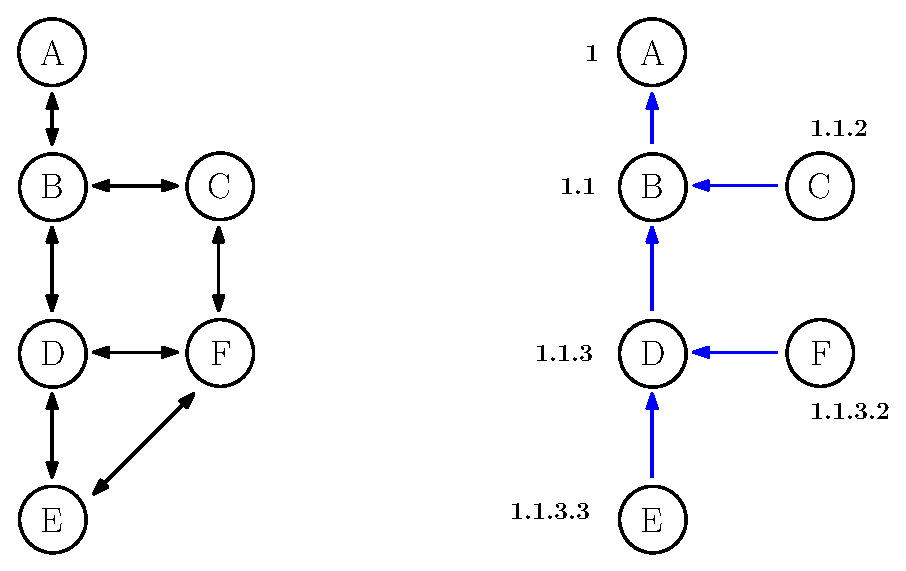
\includegraphics[width=0.7\textwidth]{fig/04_in-band/in_band_4.eps}
     \caption{Establecimiento de la topología lógica.}
     \label{fig:in_band_4}
\end{figure}


La principal ventaja de este diseño in-band es su simplicidad, en el caso más sencillo, el protocolo puede operar con una única \gls{hlmac} asignada por nodo, es decir,  una sola entrada de enrutamiento, y, aun así, ofrecer conectividad con el controlador. Además, el número de \glspl{hlmac} que requiere cada dispositivo es independiente del tamaño total de la red, además de configurable, lo que reduce drásticamente la memoria necesaria en dispositivos \gls{iot} con recursos limitados. \\
\\
En cuanto al número de mensajes intercambiados, cada nodo sólo necesita enviar un mensaje \textit{Hello} periódico y tantas transmisiones de asignación de \glspl{hlmac} como caminos \textit{multipath} se configuren; si sólo se mantiene una \gls{hlmac}, bastan únicamente dos mensajes periódicos en total. Estos intercambios están basados en eventos, y su dinámica es comparable a la difusión de un mensaje desde el nodo raíz hacia el resto de la red, proceso que suele ser rápido en comparación con protocolos de estado de enlace. Por último, la frecuencia de estas actualizaciones es configurable en función de la movilidad: escenarios con alta movilidad requieren periodos cortos, mientras que entornos estáticos pueden emplear periodos más largos.

\section{Implementación de wireless In-Band Basic OpenFlow Software Switch (win-BOFUSS)}

La implementación del protocolo se ha realizado sobre la plataforma \textit{Basic OpenFlow Software Switch} (\gls{bofuss}). Esta elección no ha sido arbitraria, ya que, en comparación con otros software-switches ampliamente utilizados, como \gls{ovs}, \gls{bofuss} ofrece un datapath cuya implementación resulta más sencilla de desarrollar y depurar, al ejecutarse en espacio de usuario y no en espacio de \textit{kernel}.\\
\\
Los orígenes de \gls{bofuss} se remontan a 2008, cuando en la Universidad de Stanford se desarrolló la primera implementación de referencia del protocolo OpenFlow, denominada \textit{The Stanford Reference OpenFlow Switch} (McKeown \textit{et al.}~\cite{mckeown2008openflow}). Dicho desarrollo constituyó un producto mínimo viable, concebido con el objetivo de demostrar el funcionamiento del protocolo y facilitar el proceso de estandarización de OpenFlow 1.0. Posteriormente, el proyecto fue retomado por los laboratorios de Ericsson, donde se amplió su funcionalidad para soportar OpenFlow 1.1 (Lajos \textit{et al.}~\cite{of11softswitch}). Años más tarde, el trabajo fue continuado por el investigador Eder Fernandes en el marco de su TFM y su tesis doctoral en Brasil~\cite{fernandes2014openflow}, consolidando lo que actualmente conocemos como \gls{bofuss}, con soporte para OpenFlow 1.3 (Fernandes \textit{et al.}~\cite{fernandes2020road}). Posteriormente, este software switch fue extendido por mi compañero de laboratorio, Constantin, quien implementó capacidades de comunicación \textit{in-band} en entornos cableados (Constantin \textit{et al.}~\cite{constantin2020desarrollo}). A partir de esta última versión, y teniendo en cuenta las lecciones aprendidas de IoTorii (Rojas \textit{et al.}~\cite{rojas2021outperforming}), se desarrolló \texttt{win-BOFUSS}, una implementación del software switch con soporte \textit{in-band} en redes inalámbricas de baja capacidad. En la Figura~\ref{fig:in_band_5} se muestra la evolución histórica del desarrollo del switch, desde su origen en 2008 con la propuesta del protocolo OpenFlow, hasta la actual implementación de \texttt{win-BOFUSS} (Carrascal \textit{et al.}~\cite{carrascal2023scalable}).

\begin{figure}[ht!]
    \centering
    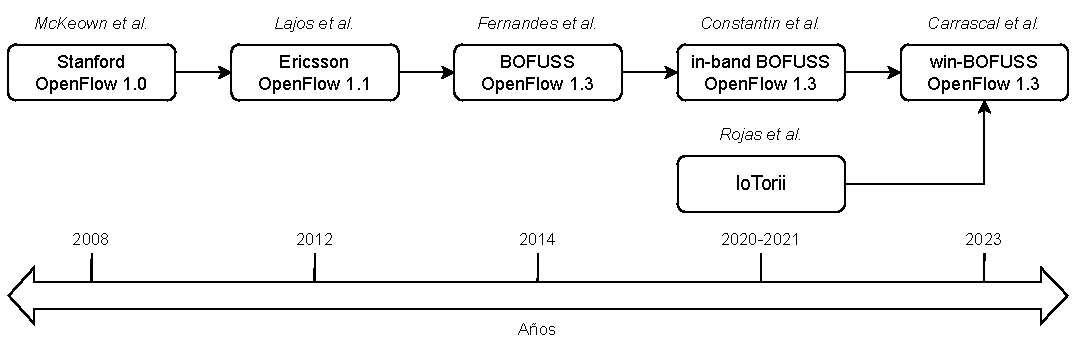
\includegraphics[width=\textwidth]{fig/04_in-band/in_band_5.drawio.pdf}
    \caption{Evolución cronológica del desarrollo del software switch BOFUSS.} 
    \label{fig:in_band_5}
\end{figure}

En la Figura~\ref{fig:in_band_6} se muestra el diagrama de flujo que recoge la implementación de la lógica del protocolo. Por defecto, \gls{bofuss} no arranca con la funcionalidad \emph{in-band} habilitada, por lo que al invocar el proceso en espacio de usuario, donde, entre otras cosas, se especifican las interfaces a gestionar, es preciso activar explícitamente la lógica \emph{in-band} mediante el parámetro \texttt{--inband}. Tras la inicialización del protocolo, el primer paso consiste en configurar los temporizadores: los asociados al envío periódico de mensajes \textit{Hello} y los vinculados a las entradas de las tablas de vecinos y de \gls{hlmac}. A continuación, cada nodo utiliza su interfaz inalámbrica para emitir el primer mensaje \textit{Hello} y así descubrir qué dispositivos se encuentran dentro de su área de cobertura, estableciendo, de ese modo, las relaciones de vecindad iniciales. Completada la fase de inicialización, el sistema entra en el bucle principal de la lógica del protocolo, que gestiona el refresco de temporizadores, la recepción y procesamiento de \textit{Hello}s y \gls{hlmac}s, y las acciones de mantenimiento de tablas y rutas.

\begin{figure}[ht!]
    \centering
    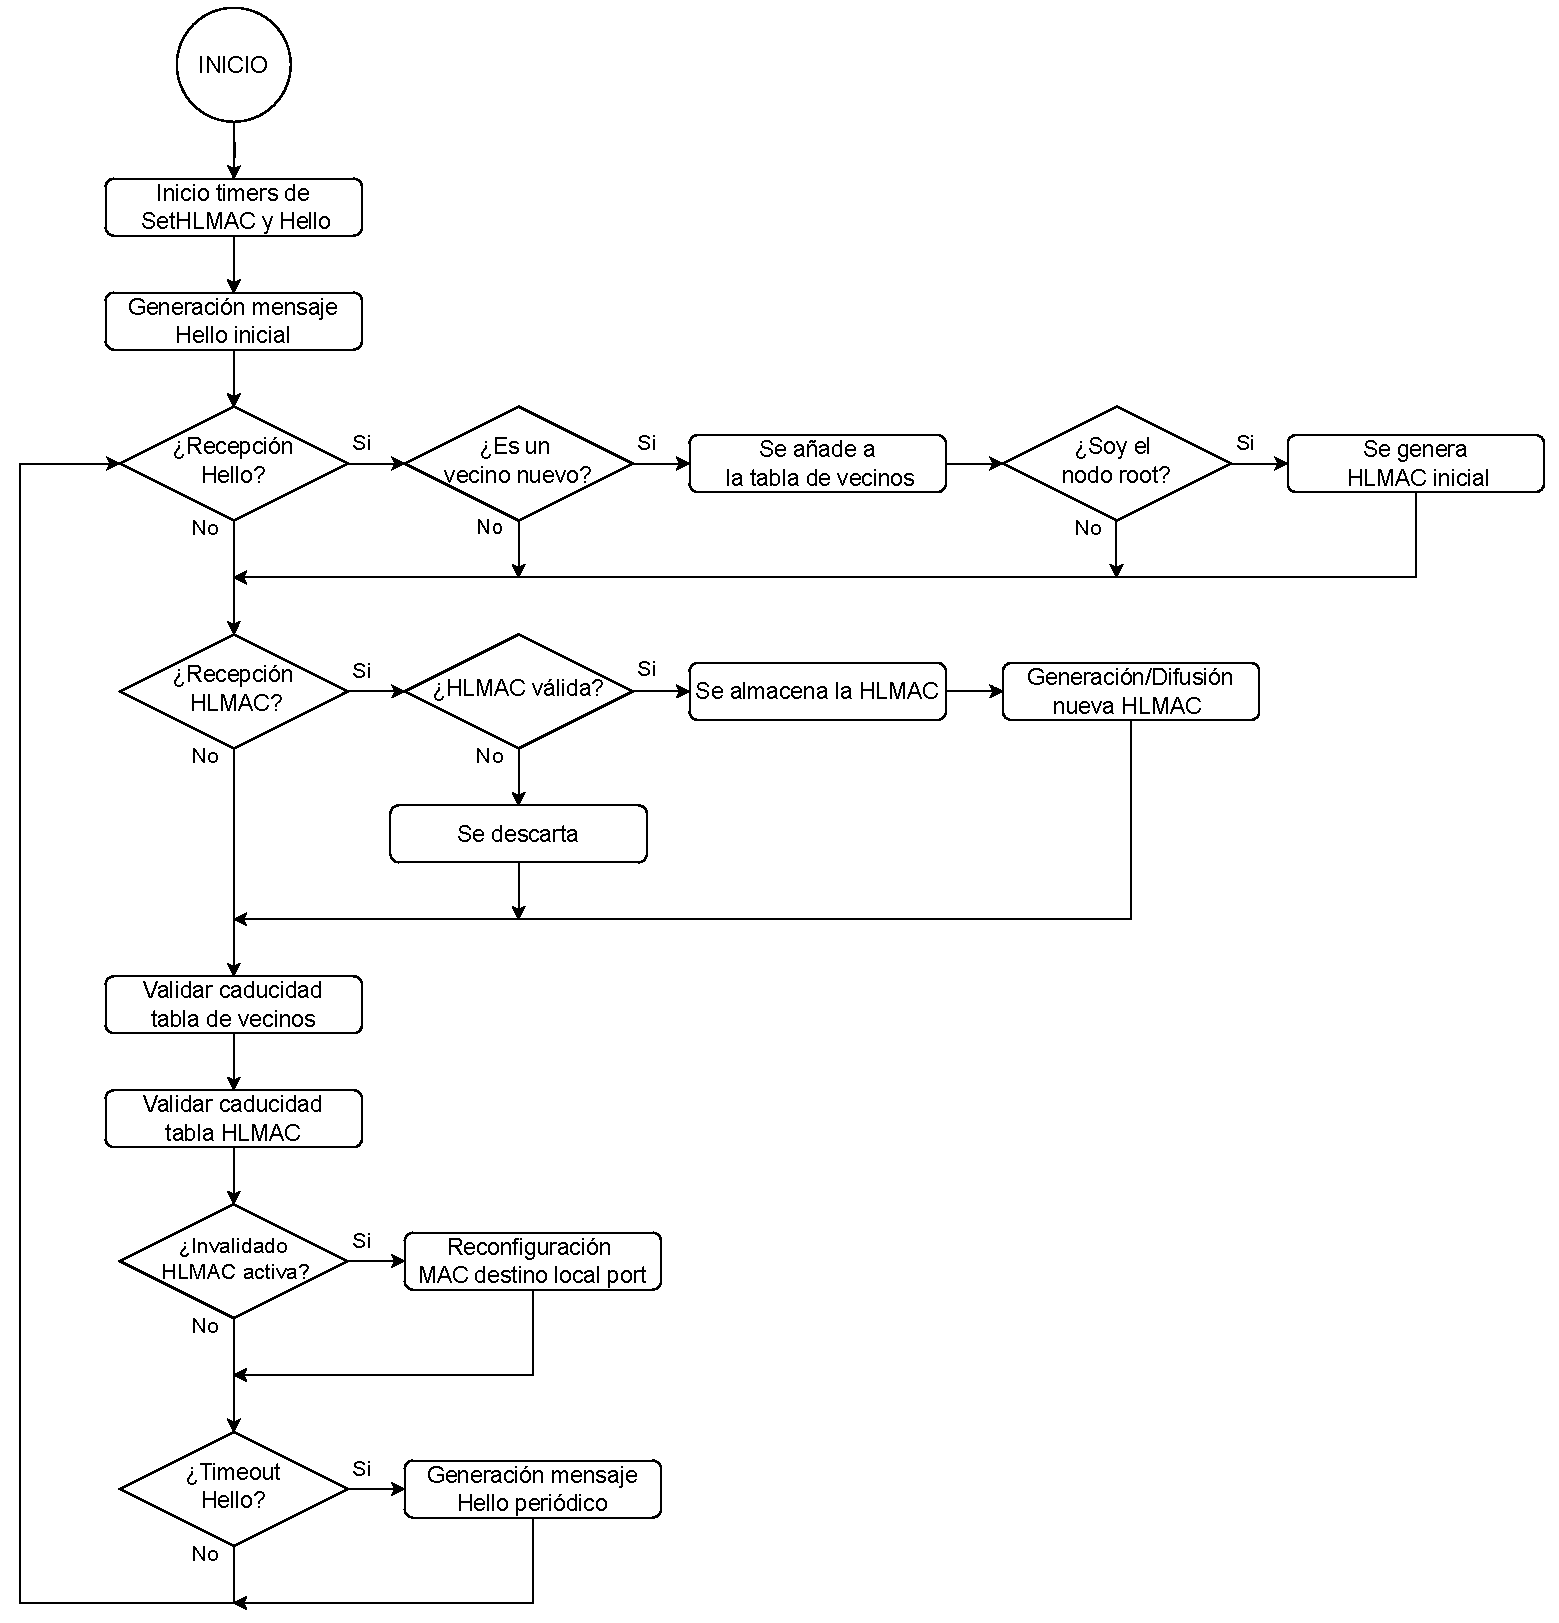
\includegraphics[width=\textwidth]{fig/04_in-band/in_band_6.drawio.pdf}
    \caption{Evolución cronológica del desarrollo del software switch BOFUSS.} 
    \label{fig:in_band_6}
\end{figure}

En el bucle principal se gestionan de forma \textit{event-driven} los siguientes sucesos: recepción de un mensaje \textit{Hello}, recepción de una \gls{hlmac}, expiración de entradas en la tabla de vecinos, expiración de entradas en la tabla de \gls{hlmac}, verificación de la ruta principal (posible reconfiguración) y vencimiento del temporizador periódico de envío de \textit{Hello}. Al recibir un \textit{Hello} se comprueba si el emisor es un vecino nuevo; en ese caso se inserta la entrada correspondiente en la tabla de vecinos y se inicia su temporizador. Si el emisor es el nodo raíz (\textit{root}), además se genera el \gls{hlmac} inicial que pone en marcha la asignación jerárquica de etiquetas en la topología. Al recibir una \gls{hlmac}, se valida que no represente un bucle; si es válida se almacena en la tabla de \gls{hlmac} y, acorde con el procedimiento descrito en la Sección~\ref{subsubsec:procesoEtiquetado}, se difunde a los hijos correspondientes. Posteriormente, se evalúan criterios para activar la dirección \gls{hlmac} preferente y se actualizan las rutas. Finalmente, en cada iteración se comprueba la caducidad de las entradas de las tablas (que se refrescan con la llegada de mensajes coincidentes) y se actúa en consecuencia: eliminar vecinos o \gls{hlmac} caducados, o forzar una reconfiguración si la ruta principal ha dejado de ser válida.\\
\\
Cuando una ruta almacenada en la tabla \gls{hlmac} deja de renovarse, es decir, el nodo correspondiente al siguiente salto deja de enviar mensajes \textit{Hello}, la entrada se invalida y el mecanismo elige la siguiente ruta disponible en la misma tabla. Dado que la interfaz física no cambia (misma interfaz inalámbrica), el puerto local permanece, pero sí varía el \textit{next-hop}: es necesario actualizar la dirección \gls{mac} de destino asociada a la IP del siguiente salto en la pila del sistema para que los paquetes salientes alcancen al nuevo vecino. En sistemas Linux esta actualización se puede realizar mediante Netlink, concretamente enviando un mensaje del tipo \texttt{RTM\_NEWNEIGH} para modificar la caché ARP (o la entrada NUD correspondiente). El procedimiento general es el siguiente: abrir un socket Netlink hacia el kernel, construir el mensaje \texttt{RTM\_NEWNEIGH} con los atributos adecuados (IP objetivo y nueva dirección \gls{mac} de enlace), enviarlo y gestionar la respuesta/confirmación del kernel. Tras esta operación, los paquetes destinados a la IP en cuestión deberán resolverse hacia la nueva \gls{mac}. En la implementación actual se ha observado una limitación práctica: la actualización de la entrada ARP no siempre es suficiente para mantener transparente una conexión TCP ya establecida con el controlador, por lo que, como solución robusta y sencilla, el prototipo vuelve a establecer la sesión TCP tras actualizar la información de \textit{next-hop}. En trabajos futuros se explorará una integración más fina (p. ej. manipulación de tablas de encaminamiento/vecindad sin interrumpir sockets existentes o el uso de opciones de kernel que permitan refrescar la resolución de enlace de forma totalmente transparente).\\
\\
Por último, se verifica el vencimiento del temporizador periódico de \textit{Hello}; si ha caducado, se emite un nuevo mensaje \textit{Hello} que refresca el estado en las tablas de los vecinos. La resiliencia del protocolo depende en gran medida de su capacidad para detectar y recuperarse con rapidez ante fallos y cambios topológicos. Ajustando adecuadamente el periodo de los \textit{Hello} y los tiempos de caducidad de las entradas, el protocolo puede identificar con rapidez enlaces caídos, nodos inalcanzables o la aparición de nuevos vecinos, reconstruir la tabla de vecinos y conmutar a rutas alternativas cuando proceda. Este mecanismo reduce el impacto de las interrupciones, acelera la convergencia de la red y optimiza el uso de los recursos disponibles.

\section{Evaluación}

El banco de pruebas elegido para llevar a cabo la prueba de concepto del protocolo es un entorno de emulación que utiliza, como biblioteca base, el software switch implementado, \texttt{win-BOFUSS}. No obstante, \gls{bofuss} no incorpora soporte inalámbrico nativo, por lo que se ha recurrido al módulo \texttt{mac80211\_hwsim} para emular el medio inalámbrico. En este escenario, cada instancia de \texttt{win-BOFUSS} combinada con \texttt{mac80211\_hwsim} actúa como un dispositivo inalámbrico \gls{iot} con una tarjeta Wi-Fi virtual, permitiendo emular escenarios inalámbricos en una única máquina física. La Figura~\ref{fig:in_band_7} ilustra la combinación de estas herramientas en una máquina. Como puede observarse, cada dispositivo \gls{iot} se emula encapsulándolo en una \textit{Network Namespace} para aislarlo (desde un punto de vista de red) del resto y forzar su comunicación mediante \texttt{mac80211\_hwsim}. Este módulo define los radios Wi-Fi de cada tarjeta virtual y solo intercambia información entre nodos que se encuentran dentro de su área de cobertura.\\
\\
Las características del medio radio (por ejemplo, limitaciones de transmisión por nodo) se configuran mediante el Traffic Controller (TC) de Linux. La información generada atraviesa las capas hasta llegar a la instancia de  \texttt{win-BOFUSS}, que implementa la lógica del protocolo propuesto. Las topologías de los escenarios se construyen mediante un conjunto de shell-scripts que definen el \textit{Network Namespace} aislado de cada dispositivo, su posición en un plano y su área de cobertura, de forma análoga a emuladores conocidos como Mininet o Mininet-WiFi~\cite{mininet-wifi}, lo que facilita la definición y despliegue de los escenarios y la integración con herramientas auxiliares (por ejemplo, trazado y representación de topologías).

\begin{figure}[ht!]
    \centering
    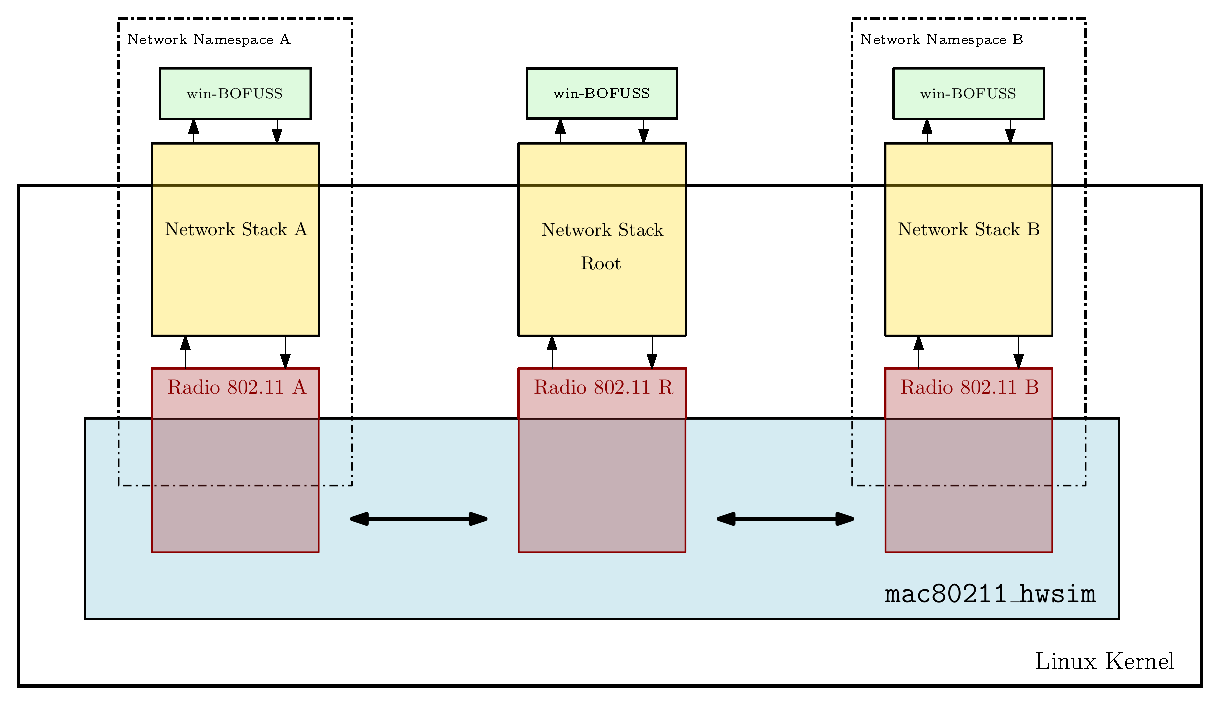
\includegraphics[width=0.95\textwidth]{fig/04_in-band/in_band_7.eps}
    \caption{Entorno de validación mediante emulación empleando el módulo del kernel \texttt{mac80211\_hwsim}.} 
    \label{fig:in_band_7}
\end{figure}

Para la prueba de concepto de nuestro protocolo de control \gls{sdn} in-band, denominado \texttt{win-BOFUSS}, se eligió la topología de la Figura~\ref{fig:in_band_3} con el fin de validar el comportamiento descrito en la Sección~\ref{sec:inband_proto_desc}. La Figura~\ref{fig:figuraCompleta} muestra dicha topología empleando las herramientas de visualización: a la izquierda el visualizador de grafos de Mininet-WiFi (Ver Figura~\ref{fig:subfiguraA}) y a la derecha el visor de topología del controlador Ryu (Ver Figura~\ref{fig:subfiguraB}). Para comprobar el funcionamiento in-band de la propuesta, el controlador \gls{sdn} Ryu se lanza en la \textit{Network Namespace} raíz, en la cual solo se encontrará corriendo uno de los nodos de la topología, por lo que el resto tendrá que valerse del mecanismo in-band implementado para alcanzar al controlador. De esta forma, ejecutando la herramienta de descubrimiento de la topología de Ryu, si el funcionamiento de la implementación de mecanismo in-band es correcto, el controlador sería capaz de descubrir todos los nodos de la topología. 

\begin{figure}[ht!]
  \centering
  \begin{subfigure}{.49\textwidth}
    \centering
    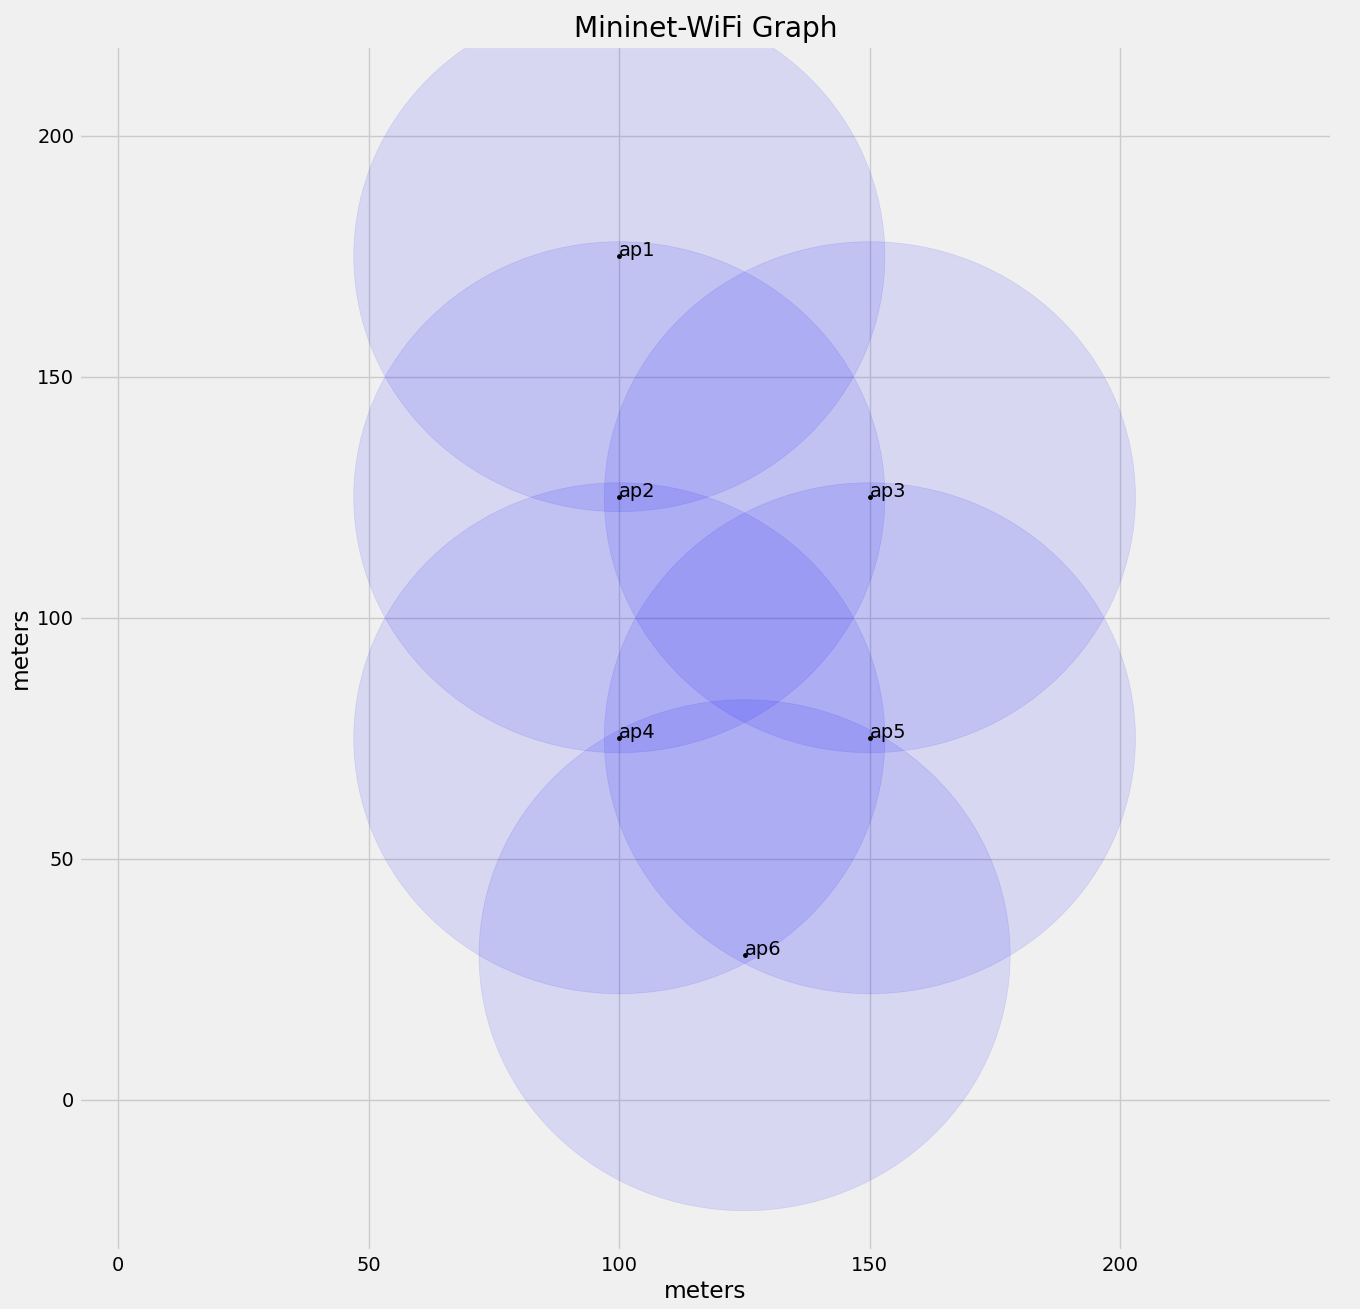
\includegraphics[width=0.9\textwidth]{fig/04_in-band/in_band_8.png}
    \caption{Topología representada por la herramienta gráfica Mininiet-WiFi.}
    \label{fig:subfiguraA}
  \end{subfigure}
  \begin{subfigure}{.49\textwidth}
    \centering
    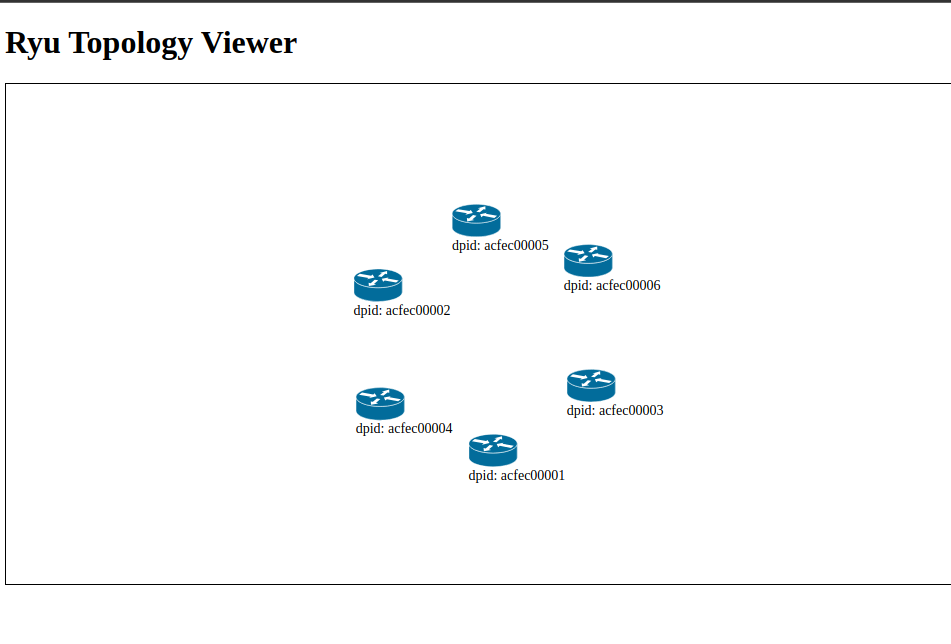
\includegraphics[width=\textwidth]{fig/04_in-band/in_band_9.png}
    \caption{Topología representada por la herramienta de descubrimiento topológico de Ryu.}
    \label{fig:subfiguraB}
  \end{subfigure}
  \caption{Topología de ejemplo elegida para el banco de pruebas.}
  \label{fig:figuraCompleta}
\end{figure}

Como puede observarse en la Figura~\ref{fig:subfiguraB}, aunque solo un dispositivo mantiene una conexión directa al controlador, este descubre correctamente el resto de los dispositivos, lo que indica que las rutas in-band se han establecido con éxito y que el diálogo OpenFlow puede iniciarse. Hay que tener en cuenta que el visor de topología de Ryu no representa las interconexiones inalámbricas entre nodos, y además no diferencia el origen de los mensajes OpenFlow de cada dispositivo cuando todos ellos llegan a través de la misma sesión (la que mantiene el nodo raíz con el controlador). Por este motivo, en la visualización de Ryu los nodos aparecen aislados y no se muestran los enlaces inalámbricos explícitamente. En cualquier caso, la topología de ejemplo queda correctamente desplegada: todos los nodos son detectados por el controlador y las rutas in-band necesarias se han configurado.\\
\\
Para analizar y verificar con mayor detalle el comportamiento del protocolo, se examinan las tablas generadas en cada dispositivo de la red. En primer lugar, se marca el nodo \textit{A} como raíz y se lanza el protocolo. Por un lado, se recopila la asociación \((MAC \rightarrow ID)\) creada en la tabla de vecinos por cada nodo tras el intercambio de mensajes \textit{Hello}. Por otro lado, se registran las \gls{hlmac} almacenadas en cada nodo tras el proceso de inundación de etiquetas. Estos resultados se muestran en la Figura~\ref{fig:figuraCompleta2}: la Figura~\ref{fig:subfiguraA2} contiene el resultado del proceso de intercambio de \textit{Hello}, y la Figura~\ref{fig:subfiguraB2} ilustra las rutas \gls{hlmac} almacenadas en cada nodo. Como puede apreciarse, el análisis teórico realizado en la Sección~\ref{sec:inband_proto_desc} coincide con los resultados experimentales. Por ejemplo, en la Figura~\ref{fig:subfiguraA2}, \textit{A} ha detectado un único vecino al que ha asignado el ID 1, que corresponde al nodo \textit{B}, tal y como en el ejemplo teórico. De igual modo, los nodos \textit{B}, \textit{D} y \textit{F} presentan tres vecinos, mientras que \textit{C} y \textit{E} muestran dos. Respecto a las rutas \gls{hlmac} almacenadas, la Figura\ref{fig:subfiguraB2} reproduce los mismos resultados que el análisis teórico: por ejemplo, \textit{D} ha almacenado las rutas \textit{1.1.3}, \textit{1.1.2.2.2} y \textit{1.1.2.2.3.1}, lo que confirma que el protocolo funciona correctamente en el escenario emulado.

\begin{figure}[ht!]
  \centering
  \begin{subfigure}{.5\textwidth}
    \centering
    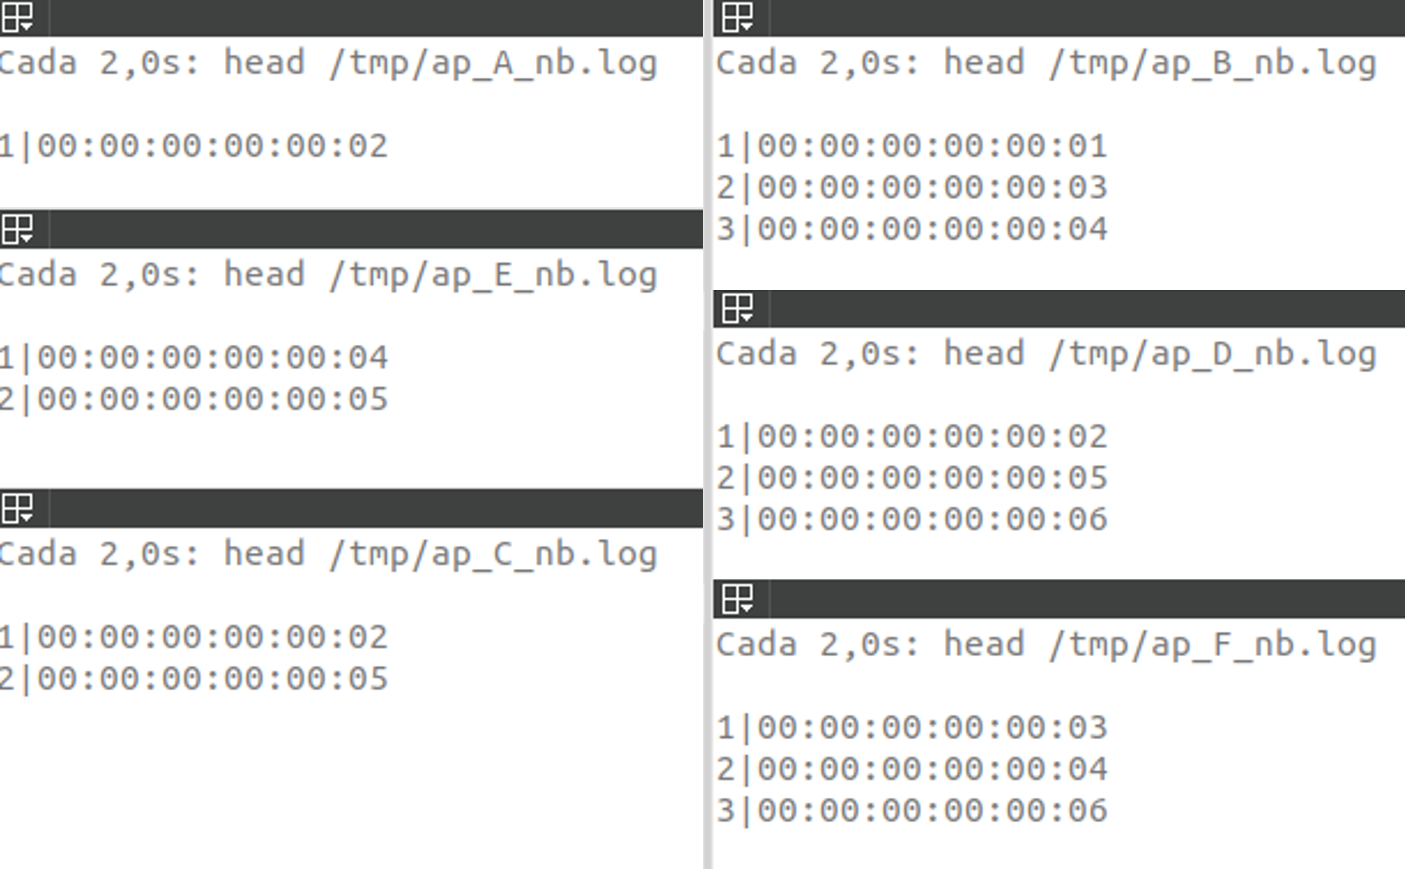
\includegraphics[width=0.95\textwidth]{fig/04_in-band/in_band_10.png}
    \caption{Neighbors table}
    \label{fig:subfiguraA2}
  \end{subfigure}%
  \begin{subfigure}{.5\textwidth}
    \centering
    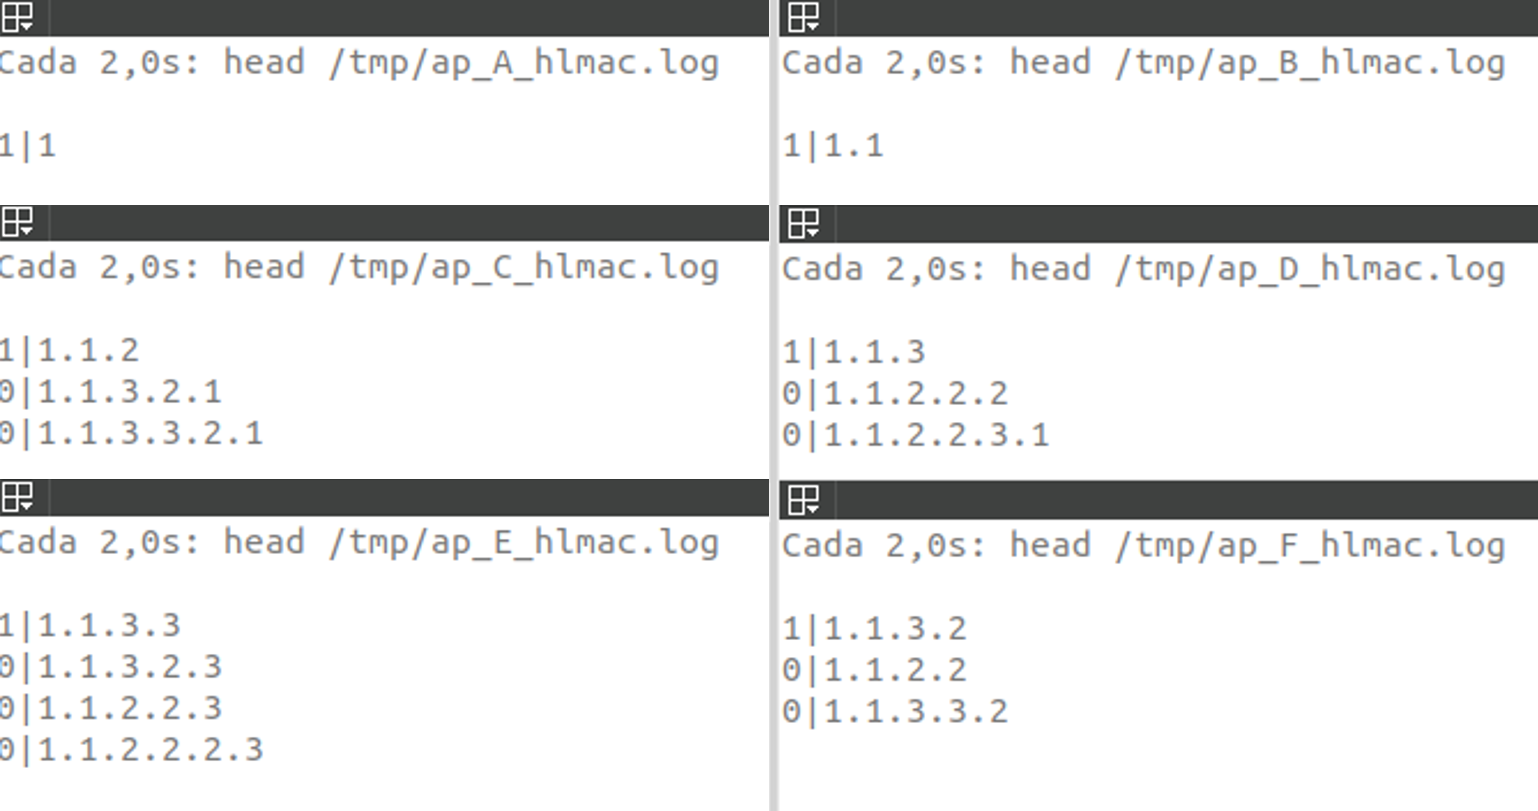
\includegraphics[width=\textwidth]{fig/04_in-band/in_band_11.png}
    \caption{HLMAC table}
    \label{fig:subfiguraB2}
  \end{subfigure}
  \caption{Functional testing of the implementation on the basic example topology.}
  \label{fig:figuraCompleta2}
\end{figure}

\section{Conclusiones}

En este trabajo hemos definido e implementado un protocolo de control in-band específicamente diseñado para su aplicación en entornos \gls{sdn} inalámbricos, prestando especial atención a los dispositivos \gls{iot} con recursos restringidos en el borde de la red. La implementación se ha integrado con éxito en el switch de referencia \gls{bofuss}, acuñándolo como \texttt{win-BOFUSS}, y se ha probado conjuntamente con la plataforma controladora Ryu. El protocolo requiere un número muy reducido de mensajes de señalización y mantiene compactas las entradas en las tablas de enrutamiento, lo que lo hace especialmente apropiado para dispositivos con capacidades de cómputo, memoria y energía limitadas. Además, ofrece mecanismos intrínsecos de resiliencia: se generan rutas de respaldo que permiten mantener la sesión de control y garantizar continuidad de servicio frente a fallos o escenarios de movilidad. En conjunto, esta aportación constituye una base sólida para futuros desarrollos orientados al despliegue del cloud continuum y al uso del etiquetado jerárquico para establecer encaminamiento autónomo.